%%%%%%%%%%%%%%%%%%%%%%%%%%%%%%%%%%%%%%%%%
% Diaz Essay
% LaTeX Template
% Version 2.0 (13/1/19)
%
% This template originates from:
% http://www.LaTeXTemplates.com
%
% Authors:
% Vel (vel@LaTeXTemplates.com)
% Nicolas Diaz (nsdiaz@uc.cl)
%
% License:
% CC BY-NC-SA 3.0 (http://creativecommons.org/licenses/by-nc-sa/3.0/)
%
%%%%%%%%%%%%%%%%%%%%%%%%%%%%%%%%%%%%%%%%%

%----------------------------------------------------------------------------------------
%	PACKAGES AND OTHER DOCUMENT CONFIGURATIONS
%----------------------------------------------------------------------------------------

\documentclass[11pt]{diazessay} % Font size (can be 10pt, 11pt or 12pt)
\usepackage{listings}
\usepackage{color}

\definecolor{miverde}{rgb}{0,0.6,0}
\definecolor{migris}{rgb}{0.5,0.5,0.5}
\definecolor{mimalva}{rgb}{0.58,0,0.82}

\lstset{ %
	backgroundcolor=\color{white},   % Indica el color de fondo; necesita que se añada \usepackage{color} o \usepackage{xcolor}
	basicstyle=\footnotesize,        % Fija el tamaño del tipo de letra utilizado para el código
	breakatwhitespace=false,         % Activarlo para que los saltos automáticos solo se apliquen en los espacios en blanco
	breaklines=true,                 % Activa el salto de línea automático
	captionpos=b,                    % Establece la posición de la leyenda del cuadro de código
	commentstyle=\color{miverde},    % Estilo de los comentarios
	deletekeywords={...},            % Si se quiere eliminar palabras clave del lenguaje
	escapeinside={\%*}{*)},          % Si quieres incorporar LaTeX dentro del propio código
	extendedchars=true,              % Permite utilizar caracteres extendidos no-ASCII; solo funciona para codificaciones de 8-bits; para UTF-8 no funciona. En xelatex necesita estar a true para que funcione.
	keepspaces=true,                 % Mantiene los espacios en el texto. Es útil para mantener la indentación del código(puede necesitar columns=flexible).
	columns=flexible,
	keywordstyle=\color{blue},       % estilo de las palabras clave
	language=Pascal,                 % El lenguaje del código
	otherkeywords={*,...},           % Si se quieren añadir otras palabras clave al lenguaje
	numbers=left,                    % Posición de los números de línea (none, left, right).
	numbersep=5pt,                   % Distancia de los números de línea al código
	numberstyle=\small\color{migris}, % Estilo para los números de línea
	rulecolor=\color{black},         % Si no se activa, el color del marco puede cambiar en los saltos de línea entre textos que sea de otro color, por ejemplo, los comentarios, que están en verde en este ejemplo
	stringstyle=\color{mimalva},     % Estilo de las cadenas de texto
	tabsize=2,	                   % Establece el salto de las tabulaciones a 2 espacios
	title=\lstname                   % muestra el nombre de los ficheros incluidos al utilizar \lstinputlisting; también se puede utilizar en el parámetro caption
}

%----------------------------------------------------------------------------------------
%	TITLE SECTION
%----------------------------------------------------------------------------------------

\title{\textbf{Aplicación big data sobre el efecto del coronavirus en el mundo}} % Title and subtitle

\author{\textbf{Bases de Datos Avanzadas} \\ \textit{Escuela Superior Informática (UCLM)}} % Author and institution

\date{\today} % Date, use \date{} for no date

%----------------------------------------------------------------------------------------

\begin{document}

\maketitle % Print the title section

%----------------------------------------------------------------------------------------
%	ABSTRACT AND KEYWORDS
%----------------------------------------------------------------------------------------

%\renewcommand{\abstractname}{Summary} % Uncomment to change the name of the abstract to something else

\begin{abstract}
	
	Este proyecto tratará sobre la creación de una aplicación \textit{big data}, para la cual se realizará un estudio sobre el efecto del coronavirus (\textbf{COVID-19}) en el mundo. Para ello se usará las diversas técnicas utilizadas para el tratamiento masivo de información

\end{abstract}

\hspace*{3.6mm}\textit{Keywords:} \textit{Big Data}, \textit{MongoDB}, \textit{Azure Cosmos DB}

\vspace{20pt} % Vertical whitespace between the abstract and first section

%----------------------------------------------------------------------------------------
%	ESSAY BODY
%----------------------------------------------------------------------------------------

\section*{Introducción}
El \textbf{Big Data} (\textit{macro datos, datos masivos, inteligencia de datos}), se conoce como el análisis masivo de datos. Esto es una cantidad de datos tan sumamente grande, que las aplicaciones que se dedicaban al  procesamiento de datos que tradicionalmente se venían usando no son capaces de tratar y poner en valor en un tiempo razonable. Este  término ha estado en uso desde la década de \textit{1990}.\\\\
Este término también hace referencia, a las nuevas tecnologías que hacen posible el almacenamiento y procesamiento de datos, además del uso que se hace de la información obtenida a través de ellas.

\subsection*{Tipos de datos que existen}
A continuación, se dará una breve explicación de los tipos de datos existentes, y de los cuales hace uso esta tecnología (\textbf{\textit{Big Data}}).

\subsubsection*{Datos estructurados}
Este tipo de datos se suelen usar en el tratamiento de datos. Ya que sus principales características son que pueden ser almacenados en tablas, y que tienen definido su formato.\\
Algunos datos de este tipo son:

\begin{itemize}
	\item \textbf{Números.}
	\item \textbf{Cadenas de caracteres.}
	\item \textbf{Fechas.}
\end{itemize}

\subsubsection*{Datos semiestructurados}
Los \textbf{\textit{datos semiestructurados}} tienen una tipo de estructura, pero esta no es lo suficientemente regular, como para permitir su gestión y estructuración como si fuese similar a los datos estructurados.
Este tipo de datos, posee ciertos patrones comunes que lo describen y dan información sobre las relaciones entre los mismos.\\\\
Un ejemplo de utilización, sería el lenguaje de marcas \textit{HTML}, el cual sirve para el desarrollo de paginas web, donde estas pautas son representadas por su sistema de etiquetas.

\subsubsection*{Datos no estructurados}
Este tipo de datos, se trata  de datos que han sido obtenidos en su formato original. Estos no se encuentran especificados en ningún formato, el cual permita que sean almacenados como se almacenarían los anteriores tipos de datos (\textit{estructurados} y \textit{semiestructurados}). Ya que no disponen de una estructura definida (longitud, formato, etc) para poder desglosar la información.\\\\
Estos datos se pueden encontrar, por ejemplo: en presentaciones (\textit{PowerPoints}), correos, documentos de texto \textit{(Word, PDF, documentos de google}, etc).

%------------------------------------------------
\newpage
\section*{Obtención de los datos}
Los datos utilizados se han obtenido de \textit{\textbf{EU Open Data Portal}} \cite{data}. El conjunto de datos contiene los últimos datos públicos disponibles sobre COVID-19, incluida una actualización diaria de la situación, la curva epidemiológica y la distribución geográfica global (UE / EEE y el Reino Unido, en todo el mundo).\\\\
Para asegurar la precisión y confiabilidad de los datos, este proceso se refina constantemente. Esto ayuda a controlar e interpretar la dinámica de la pandemia de COVID-19 no solo en la Unión Europea (UE), el Espacio Económico Europeo (EEE), sino también en todo el mundo. Todos los días, entre las 6.00 y las 10.00 CET, un equipo de epidemiólogos examina hasta 500 fuentes relevantes para recopilar las últimas cifras. El análisis de datos es seguido por el proceso estándar de inteligencia epidémica del ECDC para el cual cada entrada de datos se valida y documenta en una base de datos del ECDC \cite{ecdc}.

\clearpage

\section*{Creación de la base de datos}
La base de datos se ha construido utilizando \textit{MongoDB} \cite{mongodb} y \textit{Azure Cosmos DB} \cite{azure_cosmos}. De esta forma la base de datos es accesible desde cualquier parte. \\

MongoDB es una base de datos documental, el elemento esencial es el documento que normalmente se los agrupa en colecciones de documentos similares. Una base de datos en MongoDB es un conjunto de colecciones.\\

MongoDB almacena datos en documentos flexibles, similares a JSON, lo que significa que los campos pueden variar de un documento a otro y la estructura de datos se puede cambiar con el tiempo. El modelo de documento se asigna a los objetos en el código de su aplicación, lo que facilita el trabajo con los datos.\\

En nuestro caso, la base datos estará formada por una sola colección y el número de documentos varía con el tiempo, pero actualmente contiene más de 15000. La estructura de un documento se puede observar en la figura \ref{fig:estructura}
\begin{figure}[h!]
	\centering
	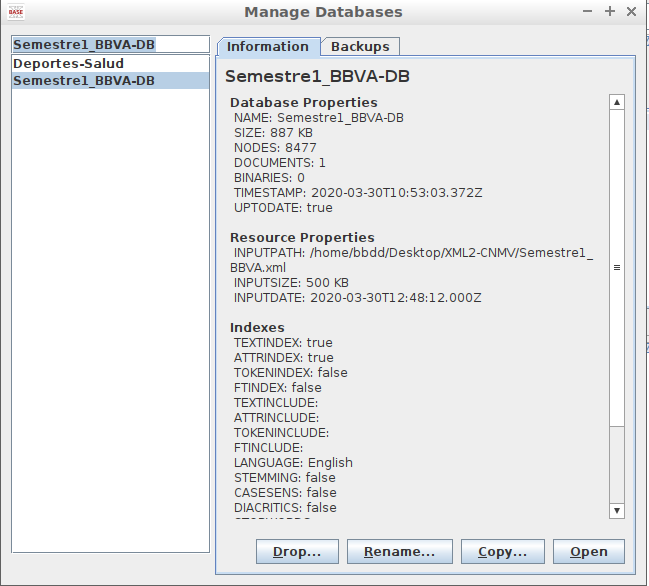
\includegraphics[width=1\linewidth]{datos}
	\caption{Estructura de un documento \cite{studio3t}}
	\label{fig:estructura}
\end{figure}

La distribución de tipos de datos se puede ver en la Figura \ref{fig:distribucion}. Siendo el tipo numérico el predominante con cinco elementos del documento de este tipo, seguido del tipo cadena con cuatro elementos y el formato fecha con un elemento. 

\begin{figure}[h!]
	\centering
	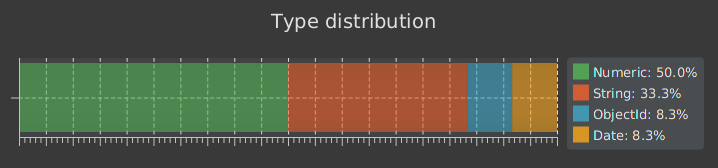
\includegraphics[width=1\linewidth]{distribucion_datos}
	\caption{Distribución de tipos de datos \cite{studio3t}}
	\label{fig:distribucion}
\end{figure}

\subsection*{Almacenamiento de datos}
Para automatizar el proceso de almacenamiento de datos hemos creado un \textit{script} en \textit{Python} \cite{python}, que descarga los datos de la fuente mencionada anteriormente en formato \textit{xlsx} y actualiza los datos en la base de datos, indicando simplemente el identificador (uri) proporcionado por \textit{Azure Cosmos DB}.\\

\lstset{language=Python}
\begin{lstlisting}
import pandas as pd
import wget
import os
from pymongo import MongoClient

url = 'https://www.ecdc.europa.eu/sites/default/files' \
'/documents/COVID-19-geographic-disbtribution-worldwide.xlsx'


def excel_to_json():
	filename = wget.download(url)
	data = pd.read_excel(filename)
	os.remove(filename)
	return data.to_dict('records')


def upload_data(uri):
	client = MongoClient(uri)
	database = client['covid']
	collection = database['Worldwide']
	collection.drop()
	collection.insert_many(excel_to_json())


upload_data(os.sys.argv[1])
\end{lstlisting}

De esta forma, cada día ejecutamos el \textit{script} y actualizamos los datos de la base de datos en cuestión de minutos, ya que como hemos comentado anteriormente los datos de la fuente se actualizan a diario.





\clearpage

\section*{Ejecución de consultas}
La ejecución de consultas la hemos realizado gracias a la creación de una clase \textit{Python}, con la cual, crearemos objetos que nos permitirán conectar fácilmente con la base de datos y obtener datos específicos por país, fecha o continente. Esta clase se comporta de forma similar a un agente, utilizado en otras asignaturas para realizar la conexión con la base de datos.

\lstset{language=Python}
\begin{lstlisting}
from pymongo import MongoClient


def parse_date(date):
	date = date.split("/")
	day = int(date[0])
	month = int(date[1])
	year = int(date[2])
	
	return day, month, year


class CovidClient:
	def __init__(self, dir_bd, name_bd, collection):
		self.__collection = MongoClient(dir_bd)[name_bd][collection]
	
	def get_total_deaths_country(self, country):
		try:
			data = self.__collection.find({"countriesAndTerritories": country}, {"deaths"})
			deaths = 0
			
			for x in data:
				deaths += int(x['deaths'])
			
			return deaths
		except Exception as e:
			return e
	
	def get_total_deaths_continent(self, continent):
		try:
			data = self.__collection.find({"continentExp": continent}, {"deaths"})
			deaths = 0
			
			for x in data:
				deaths += int(x['deaths'])
			
			return deaths
		except Exception as e:
			return e
	
	def get_total_cases_country(self, country):
		try:
			data = self.__collection.find({"countriesAndTerritories": country}, {"cases"})
			cases = 0
			
			for x in data:
			cases += int(x['cases'])
			
			return cases
		except Exception as e:
			return e
	
	def get_total_cases_continent(self, continent):
		try:
			data = self.__collection.find({"continentExp": continent}, {"cases"})
			cases = 0
			
			for x in data:
				cases += int(x['cases'])
		
			return cases
		except Exception as e:
			return e
	
	def get_worst_day_country(self, country):
		try:
			data = self.__collection.find({"countriesAndTerritories": country}, {"deaths", "dateRep"})
			deaths = None
			date = None
			
			for x in data:
				if deaths is None:
					deaths = int(x['deaths'])
					date = x['dateRep']
				else:
					if int(x['deaths']) > deaths:
						deaths = int(x['deaths'])
						date = x['dateRep']
			
			return date, deaths
		except Exception as e:
			return e
	
	def get_total_deaths(self):
		try:
			data = self.__collection.find({}, {"deaths"})
			deaths = 0
			
			for x in data:
				deaths += int(x['deaths'])
			
			return deaths
		except Exception as e:
			return e
	
	def get_total_cases(self):
		try:
			data = self.__collection.find({}, {"cases"})
			cases = 0
			
			for x in data:
				cases += int(x['cases'])
			
			return cases
		except Exception as e:
			return e
	
	def get_data_date_country(self, country, date):
		try:
			day, month, year = parse_date(date)
			data = self.__collection.find(
			{
				"countriesAndTerritories": country,
				"day": day,
				"month": month,
				"year": year
			},
			{"countriesAndTerritories", "cases", "deaths"}
			)
		
			return data
		except Exception as e:
			return e
	
	def get_data_country(self, country):
		try:
			# only days with cases or deaths
			data = self.__collection.find({"countriesAndTerritories": country,"$or": [{"cases": {"$gt": 0}},{"deaths": {"$gt": 0}}]},{"countriesAndTerritories", "cases", "deaths", "dateRep"})
			
			return data
		except Exception as e:
			return e
\end{lstlisting}

Gracias a esta clase podremos realizar multitud de consultas interesantes a la base de datos, algunas de ellas las mostraremos a continuación.

\newpage
\section*{Ejemplos de consultas}
A continuación, se realizará una serie de consultas, las cuales hemos utilizado para llevar a cabo en el estudio de la pandemia. Cabe destacarr que estos datos han sido obtenidos el día \textit{\textbf{7 de Mayo del 2020}}.\\

\subsection*{Total de casos confirmados}
Para ello se ha utilizado la función \textit{\textbf{get-total-cases()}} \cite{jupyter} de la clase \textit{CovidClient}.

\lstset{language=Python}
\begin{lstlisting}
	def get_total_cases(self):
		try:
			data = self.__collection.find({}, {"cases"})
			cases = 0
			
			for x in data:
			cases += int(x['cases'])
			
			return cases
		except Exception as e:
			return e
\end{lstlisting}

El \textbf{resultado} de la consulta sería el siguiente: \textbf{3623803} \textit{casos confirmados} en todo el mundo.


\subsection*{Total de muertes confirmadas}
Para ello se ha utilizado la función \textit{\textbf{get-total-deaths()}} \cite{jupyter} de la clase \textit{CovidClient}.

\lstset{language=Python}
\begin{lstlisting}
	def get_total_deaths(self):
		try:
			data = self.__collection.find({}, {"deaths"})
			deaths = 0
	
			for x in data:
			deaths += int(x['deaths'])
			
			return deaths
		except Exception as e:
			return e
\end{lstlisting}

El \textbf{resultado} de la consulta sería el siguiente: \textbf{256880} \textit{muertes confirmadas} en el mundo.


\newpage
\subsection*{Casos confirmados en España el mes de Marzo}
Para ello se ha utilizado la función \textit{\textbf{get-data-country()}} \cite{jupyter} de la clase \textit{CovidClient}.

\lstset{language=Python}
\begin{lstlisting}
	data = client.get_data_country('Spain')
	month = 3
	cases = []
	dates = []
	
	# Get data
	for d in data:
		date = d['dateRep']
		if date.month == month:
			cases.append(abs(d['cases']))
			dates.append(date.strftime("%d/%m"))
	
	# Reverse data
	cases = cases[::-1]
	dates = dates[::-1]
	y_pos = np.arange(len(dates))
	plt.bar(y_pos, cases)
	plt.xticks(y_pos, dates, rotation = 90)
	plt.show()
\end{lstlisting}

El \textbf{resultado} de la consulta sería el diagrama de barras de la Figura \ref{fig:spain-march} recaudando dicha información.

\begin{figure}[h!]
	\centering
	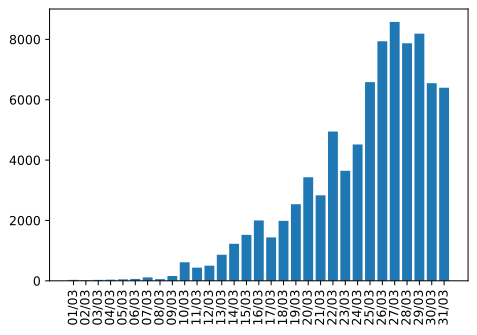
\includegraphics[width=\linewidth]{spain.png}
	\caption{Casos en España mes de Marzo. \cite{jupyter}}
	\label{fig:spain-march}
\end{figure}

\newpage
\subsection*{Muertes en Italia en el mes de Abril}
Para ello se ha utilizado la función \textit{\textbf{get-data-country()}} \cite{jupyter} de la clase \textit{CovidClient}.

\lstset{language=Python}
\begin{lstlisting}
	data = client.get_data_country('Italy')
	month = 4
	deaths = []
	dates = []
	
	for d in data:
		date = d['dateRep']
		if date.month == month:
			deaths.append(abs(d['deaths']))
			dates.append(date.strftime("%d/%m"))
	
	# Reverse data
	deaths = deaths[::-1]
	dates = dates[::-1]
	y_pos = np.arange(len(deaths))
	plt.bar(y_pos, deaths)
	plt.xticks(y_pos, dates, rotation = 90)
	plt.show()
\end{lstlisting}

El \textbf{resultado} de la consulta sería el diagrama de barras de la Figura \ref{fig:eeuu} recaudando dicha información.

\begin{figure}[h!]
	\centering
	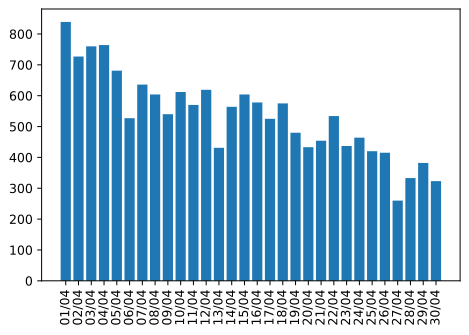
\includegraphics[width=\linewidth]{eeuu.png}
	\caption{Muertes en Italia en el mes de Abril \cite{matplotlib}}
	\label{fig:eeuu}
\end{figure}

\newpage
\subsection*{Casos confirmados agrupados por meses en Italia}
Para ello se ha utilizado la función \textit{\textbf{get-data-country()}} \cite{jupyter} de la clase \textit{CovidClient}.

\lstset{language=Python}
\begin{lstlisting}
	data = client.get_data_country('Italy')
	months = {1:0, 2:0, 3:0, 4:0, 5:0}
	
	for d in data:
		months[d['dateRep'].month] += abs(d['cases'])
	
	y_pos = np.arange(len(months.values()))
	plt.bar(y_pos, months.values())
	plt.xticks(y_pos, months.keys())
	plt.show()
\end{lstlisting}

El \textbf{resultado} de la consulta sería el diagrama de barras de la Figura \ref{fig:italy} recaudando dicha información.

\begin{figure}[h!]
	\centering
	
\includegraphics[width=10cm]{italy-months.png}
	\caption{Casos confirmados agrupados por meses en Italia. \cite{matplotlib}}
	\label{fig:italy}
\end{figure}


\subsection*{Porcentaje de casos en Estados Unidos respecto al resto del mundo}
Para ello se ha utilizado la función \textit{\textbf{get-total-cases-country()}} y \textit{\textbf{get-total-cases()}} \cite{jupyter} de la clase \textit{CovidClient}.

\lstset{language=Python}
\begin{lstlisting}
	country = "United_States_of_America"
	country_cases = client.get_total_cases_country(country)
	total_cases = client.get_total_cases() - country_cases
	
	values = [total_cases, country_cases]
	names = ["Rest of world cases", (country.replace("_"," ") + "'s cases")]
	plt.pie(values, labels=names, autopct="%0.2f %%")
	plt.show()
\end{lstlisting}

El \textbf{resultado} de la consulta sería el diagrama de barras de la Figura \ref{fig:italy} recaudando dicha información.

\begin{figure}[h!]
	\centering
	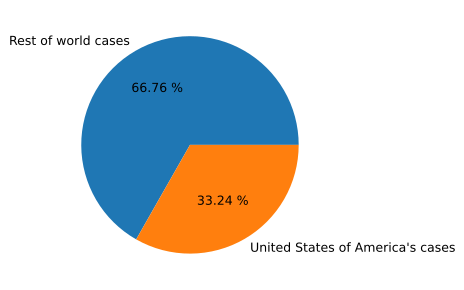
\includegraphics[width=9cm]{eeuu-plait.png}
	\caption{Porcentaje de casos en Estados Unidos respecto al resto del mundo. \cite{matplotlib}}
	\label{fig:eeuu-plait}
\end{figure}



\subsection*{Porcentaje de casos de los tres países europeos más afectados}
Para ello se ha utilizado la función \textit{\textbf{get-total-cases-country()}} y \textit{\textbf{get-total-cases-continent()}} \cite{jupyter} de la clase \textit{CovidClient}.

\lstset{language=Python}
\begin{lstlisting}
	continent = "Europe"
	country1 = "Spain"
	country2 = "Italy"
	country3 = "United_Kingdom"
	
	country1_cases = client.get_total_cases_country(country1)
	country2_cases = client.get_total_cases_country(country2)
	country3_cases = client.get_total_cases_country(country3)
	continent_cases = client.get_total_cases_continent(continent) - (country1_cases - country2_cases - country3_cases)
	
	values = [continent_cases, country1_cases, country2_cases, country3_cases]
	names = [("Rest of " + continent.replace("_", " ") + "'s cases"), (country1.replace("_"," ") + "'s cases"), (country2.replace("_"," ") + "'s cases"), (country3.replace("_"," ") + "'s cases")]
	plt.pie(values, labels=names, autopct="%0.2f %%")
	plt.show()
\end{lstlisting}

El \textbf{resultado} de la consulta sería el diagrama de barras de la Figura \ref{fig:italy} recaudando dicha información.
\clearpage

\begin{figure}[h!]
	\centering
	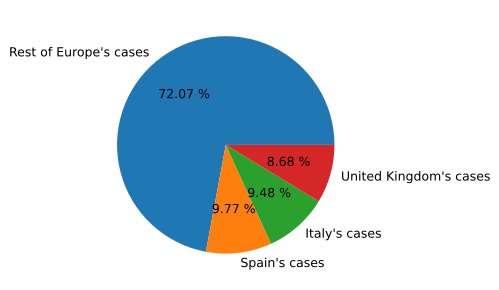
\includegraphics[width=8.5cm]{europe-plait.png}
	\caption{Porcentaje de casos de los tres países europeos más afectados. \cite{matplotlib}}
	\label{fig:europe-plait}
\end{figure}


\subsection*{Porcentaje de muertes de los tres países más afectados en el mundo}
Para ello se ha utilizado la función \textit{\textbf{get-total-deaths-country()}} y \textit{\textbf{get-total-deaths()}} \cite{jupyter} de la clase \textit{CovidClient}.

\lstset{language=Python}
\begin{lstlisting}
	country1 = "United_States_of_America"
	country2 = "Spain"
	country3 = "Italy"
	country1_deaths = client.get_total_deaths_country(country1)
	country2_deaths = client.get_total_deaths_country(country2)
	country3_deaths = client.get_total_deaths_country(country3)
	total_cases = client.get_total_deaths() - (country1_deaths - country2_deaths - country3_deaths)
	
	values = [total_cases, country1_deaths, country2_deaths, country3_deaths]
	names = ["Rest of world deaths", (country1.replace("_"," ") + "'s deaths"), (country2.replace("_"," ") + "'s deaths"), (country3.replace("_", " ") + "'s deaths")]
	plt.pie(values, labels=names, autopct="%0.2f %%")
	plt.show()
\end{lstlisting}

El \textbf{resultado} de la consulta sería el diagrama de barras de la Figura \ref{fig:italy} recaudando dicha información.

\begin{figure}[h!]
	\centering
	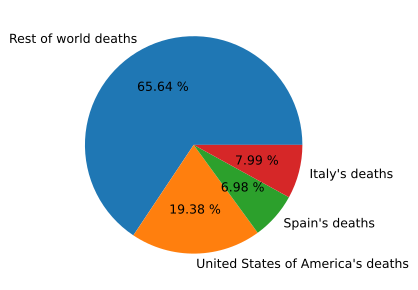
\includegraphics[width=8cm]{world-plait.png}
	\caption{Porcentaje de muertes de los tres países más afectados en el mundo. \cite{matplotlib}}
	\label{fig:world-plait}
\end{figure}

\clearpage


%Cras gravida, est vel interdum euismod, tortor mi lobortis mi, quis adipiscing elit lacus ut orci. Phasellus nec fringilla nisi, ut vestibulum neque. Aenean non risus eu nunc accumsan condimentum at sed ipsum.
%\begin{wrapfigure}{l}{0.42\textwidth} % Inline image example, use an 'r' column type to position the figure on the right
%	
\includegraphics[width=\linewidth]{fish.png}
%	\caption{An example fish.}
%\end{wrapfigure}
%Aliquam fringilla non diam sed varius. Suspendisse tellus felis, hendrerit non bibendum ut, adipiscing vitae diam. Lorem ipsum dolor sit amet, consectetur adipiscing elit. Nulla lobortis purus eget nisl scelerisque, commodo rhoncus lacus porta. Vestibulum vitae turpis tincidunt, varius dolor in, dictum lectus. Aenean ac ornare augue, ac facilisis purus. Sed leo lorem, molestie sit amet fermentum id, suscipit ut sem. Vestibulum orci arcu, vehicula sed tortor id, ornare dapibus lorem. Praesent aliquet iaculis lacus nec fermentum. Morbi eleifend blandit dolor, pharetra hendrerit neque ornare vel. Nulla ornare, nisl eget imperdiet ornare, libero enim interdum mi, ut lobortis quam velit bibendum nibh.
%
%\begin{itemize}
%	\item First bullet point item
%	\item Second bullet point item
%	\item Third bullet point item
%\end{itemize}
%
%Morbi tempor congue porta. Proin semper, leo vitae faucibus dictum, metus mauris lacinia lorem, ac congue leo felis eu turpis. Sed nec nunc pellentesque, gravida eros at, porttitor ipsum. Praesent consequat urna a lacus lobortis ultrices eget ac metus. In tempus hendrerit rhoncus. Mauris dignissim turpis id sollicitudin lacinia. Praesent libero tellus, fringilla nec ullamcorper at, ultrices id nulla. Phasellus placerat a tellus a malesuada.
%
%\begin{enumerate}
%	\item First numbered list item
%	\item Second numbered list item
%\end{enumerate}

%------------------------------------------------

%\section*{Conclusion}
%
%Fusce in nibh augue. Cum sociis natoque penatibus et magnis dis parturient montes, nascetur ridiculus mus. In dictum accumsan sapien, ut hendrerit nisi. Phasellus ut nulla mauris. Phasellus sagittis nec odio sed posuere. Vestibulum porttitor dolor quis suscipit bibendum. Mauris risus lectus, cursus vitae hendrerit posuere, congue ac est. Suspendisse commodo eu eros non cursus. Mauris ultrices venenatis dolor, sed aliquet odio tempor pellentesque. Duis ultricies, mauris id lobortis vulputate, tellus turpis eleifend elit, in gravida leo tortor ultricies est. Maecenas vitae ipsum at dui sodales condimentum a quis dui. Nam mi sapien, lobortis ac blandit eget, dignissim quis nunc.
%
%Donec luctus tincidunt mauris, non ultrices ligula aliquam id. Sed varius, magna a faucibus congue, arcu tellus pellentesque nisl, vel laoreet magna eros et magna. Vivamus lobortis elit eu dignissim ultrices. Fusce erat nulla, ornare at dolor quis, rhoncus venenatis velit. Donec sed elit mi. Sed semper tellus a convallis viverra. Maecenas mi lorem, placerat sit amet sem quis, adipiscing tincidunt turpis. Cras a urna et tellus dictum eleifend. Fusce dignissim lectus risus, in bibendum tortor lacinia interdum.
%
%\begin{table}[h] % [h] forces the table to be output where it is defined in the code (it suppresses floating)
%	\caption{Example table.}
%	\centering
%	\begin{tabular}{l l r}
%		\toprule
%		\multicolumn{2}{c}{Name} \\
%		\cmidrule(r){1-2}
%		First Name & Last Name & Grade \\
%		\midrule
%		John & Doe & $7.5$ \\
%		Richard & Miles & $5$ \\
%		\bottomrule
%	\end{tabular}
%\end{table}
%
%Fusce eleifend porttitor arcu, id accumsan elit pharetra eget. Mauris luctus velit sit amet est sodales rhoncus. Donec cursus suscipit justo, sed tristique ipsum fermentum nec. Ut tortor ex, ullamcorper varius congue in, efficitur a tellus. Vivamus ut rutrum nisi. Phasellus sit amet enim efficitur, aliquam nulla id, lacinia mauris. Quisque viverra libero ac magna maximus efficitur. Interdum et malesuada fames ac ante ipsum primis in faucibus. Vestibulum mollis eros in tellus fermentum, vitae tristique justo finibus. Sed quis vehicula nibh. Etiam nulla justo, pellentesque id sapien at, semper aliquam arcu. Integer at commodo arcu. Quisque dapibus ut lacus eget vulputate.

%----------------------------------------------------------------------------------------
%	BIBLIOGRAPHY
%----------------------------------------------------------------------------------------

\bibliographystyle{abbrv}

\bibliography{sample.bib}

%----------------------------------------------------------------------------------------

\end{document}
